%\documentclass[twocolumn,prb,superscriptaddress,amsmath,amssymb,aps,floatfix]{revtex4}
\documentclass[twocolumn,amsmath, floatfix]{revtex4}
%\usepackage{amsmath}
%\usepackage{bm}
%\usepackage{braket}
%\usepackage{graphicx,subcaption}
%\usepackage{graphicx,subfigure}
\usepackage{graphicx}
\usepackage{float}
\usepackage{siunitx}
\usepackage{caption}
%\usepackage{color}
%\usepackage{url}
%\usepackage[latin1]{inputenc}
%\usepackage{tikz}
%\usepackage[toc,page]{appendix}
%\makeatletter
%\def\BState{\State\hskip-\ALG@thistlm}
%\makeatother

\begin{document}
\title { Semi-automated segmentation of atomic-resolution microscopy images with unsupervised machine learning}
\author{Ning~Wang}
\affiliation{Max-Planck-Institut f{\"u}r Eisenforschung GmbH,  Max-Planck-Stra{\ss}e 1, 40237 D{\"u}sseldorf, Germany }
\author{Christoph~Freysoldt}
\affiliation{Max-Planck-Institut f{\"u}r Eisenforschung GmbH,  Max-Planck-Stra{\ss}e 1, 40237 D{\"u}sseldorf, Germany }
\author{Christian~Liebscher}
\affiliation{Max-Planck-Institut f{\"u}r Eisenforschung GmbH,  Max-Planck-Stra{\ss}e 1, 40237 D{\"u}sseldorf, Germany }
\begin{abstract}

We present an unsupervised machine learning approach for semi-automated segmentation of 
atomic-resolution microscopy images. 
We combine our newly-proposed symmetry-based local descriptors with the classical unsupervised machine learning algorithms, and highlight that the microscopy images might be segmented in an unsupervised manner bypassing the tedious training of supervised machine learning models.
We demonstrate in this paper the applications to the high-angle annular dark-field scanning Transmission electron microscopy (HAADF-STEM) images, while the approach is of general applicability to atomic-resolution microscopy images. 
Our code is released as a python module, which reads the microscopy images and outputs the labels for all pixels. 
\end{abstract}

\maketitle

\section{Introduction}
The development of materials science is largely driven by that of microscopes. Since the second half of the last century, the substantial advances of microscopy have made it possible to probe materials with atomic resolution \cite{Hansma209}, which opens up an era where the materials can be studied down to the level of singe atoms. 
Accompanying the ubiquitous acquisition of data at the atomic scale, we are facing the challenge of efficiently analyzing the large amount of data generated even in a single experiment \cite{Sergei2015}. The machine-learning methods have been shown to be effective in speeding up and automatizing the data processing in various microscopy-related problems \cite{Kaufmann2020,Sergei2019, Sergei2020}.

The high-resolution imaging microscopes, such as STEM, have made it routine to acquire atomic-resolution images and videos. To analyze the large volume of microscopy images becomes a tedious task for researchers, and the manual imaging analysis has the drawback of inconsistency in interpreting the image either qualitatively or quantitatively. Among various image analysis tasks, the image segmentation is crucial as it relates the digital signals to crystal patterns and serve as a necessary step for further analysis, and challenging as each pixel in the image needs to be interpreted correctly according to the features of its local surroundings and linked to the correct pattern label.  The recent substantial advances of machine learning and computer vision provides powerful tools to resolve this challenge and aid us to develop the efficient and robust approach for the segmentation of atomic-resolution microscopy images, which is the focus of this paper.

As the difference between the crystal patterns in the atomic-resolution images are dominated by the arrangement of atoms, the conventional segmentation methods such as thresholding \cite{Sadowski2006, Mancas2005} and region merging \cite{Navlakha2013,Nock2004} are not straightforwardly applicable for this task.  The supervised machine learning methods \cite{Ignacio2017, Dang2019} have been explored in the community of biology to segment the tissue images, which require a large amount of labeled data to train a classification model or a neural network. While the good progress has been demonstrated in literature, the drawback of the supervised models are also transparent. The data labeling is time-consuming and the supervised model has no general applicability and only works for the images that are similar to those in training data. Our approach is based on the consideration that the segmentation of atomic-resolution images is mostly based on the local symmetry, which might be encoded into the local descriptors. The local descriptors can then be fed into the unsupervised clustering algorithms in order to segment the microscopy images. The closest work to ours is probably the machine learning-based workflow for segmentation of atomic force microscopy (AFM) images that was published by Borodinov et al.\cite{Borodinov2020} very recently.  In their workflow, the local descriptors are first calculated with a pre-selected transform (Discrete Fourier, wavelet, or Radon transform), which are fed into the clustering algorithms to segment the AFM images.
Our approach shares the similar architecture with their workflow. 
What makes our work different stem from several aspects. We exploit the self-similarity inherent in the microscopy images and propose the symmetry-based local descriptors. We find that an up-sampling plus stride scheme effective to speed up the segmentation. We further package our code as a python module, which is ready to use simply by typing several lines of python code and flexible to be plugged into other microscopy packages.   \\
Our segmentation approach consists of four steps:\\
1. calculate the symmetry-based local descriptors;\\
2 perform principle component analysis to reduce the dimension;\\
3. perform K-means clustering in the descriptor space;\\
4. perform up-sampling to match the shape of the original image.\\
There are several hyperparameters to be specified by the users, and this is the reason why we claim our approach to be semi-automated. Once the hyperparameters are specified, all of the rest are performed by the computer automatically. 
%In this paper, we propose to employ the symmetry operations to extract the local-symmetry features. 
%we proposed three types of local descriptors that encode the translational, rotational, or reflectional symmetry, respectively, and showed that they can be combined with the K-means clustering algorithm and an up-sampling scheme to efficiently segment the atomic-resolution images in a semi-automated and unsupervised manner.

Next, we explain each step of our approach in the methodology section, and in the application section, we present two examples of the application to HAADF-STEM images.
%The paper is structured as follows. In the methodology section, 
%We first introduce our self-similarity-based local descriptors. After that we briefly review the K-means clustering algorithm and demonstrate that it can be combined with our newly-proposed local descriptors to segment the atomic-resolution microscopy images. We finalize the methodology section by presenting two schemes to speed up the segmentation, the principle component analysis (PCA) and the up-sampling. 


\section{Methodology}
\subsection{Feature extraction via symmetry operations}
We aim at segmenting the microscopy images into multiple crystal patterns that are different in terms of symmetry, i.e., the partitions are invariant with respect to different symmetry operations.  Four types of symmetry operations are involved in the two-dimensional crystal patterns, translations, rotations, reflections, and glide-reflections, and they are dictated by the relations below,
\begin{equation}
\begin{aligned}
   & \mathrm{translation : \,\,} \mathbf{r}^\prime = \mathbf{r} + \mathbf{t}, \\
   & \mathrm{rotation: \,\,} \mathbf{r}^\prime = \mathbf{R}\mathbf{r}, \\
   & \mathrm{reflection: \,\,} \mathbf{r}^\prime = \mathbf{M}\mathbf{r}, \\
   & \mathrm{glide-reflection: \,\,} \mathbf{r}^\prime = \mathbf{M}\mathbf{r} + \mathbf{t},\\
\end{aligned}
\end{equation}
where $\mathrm{r}$ and $\mathbf{r}^\prime$ are the positions of the original and the transformed pixels,  $\mathbf{t}$ the translation vector, $\mathbf{R}$ the rotation matrix, and $\mathbf{M}$ the reflection matrix.
As the entries in translation vector and the rotation and reflection matrices may take various values, there are many possible symmetry operations. 
We choose one from them, and denote it as the candidate symmetry operation. If we apply it to a crystal pattern and score the similarity between the original and the transformed ones, the score would be high if it is the symmetry operation of the examined the pattern and low if it is not. The scoring of a series of candidate symmetry operations gives us a symmetry-score vector, which can be used as a descriptor to characterize the symmetry of the pattern. In the segmentation task, since we need to examine the local symmetry in the microscopy image, we simply apply the symmetry operations to the patches instead of the whole image, and then use the symmetry-score vector as the local descriptor.
In other words, the candidate symmetry operation together with the symmetry scoring makes a local-symmetry-feature extractor.  We shift the extractor across the whole image in order to extract the local-symmetry information everywhere in the image. The schematic diagram for this calculation is shown in Fig. \ref{local_descriptors}. 
%the local descriptors are obtained via scoring the local self-similarity with respect to the candidate symmetry operations.  \ref{local_descriptors}. 


%There are still three problems to resolve before we get the local descriptors of practical use: 1. how to define the similarity score? 2. how to choose the candidate symmetry operations? 3. how to guarantee the translational invariance?  
%In the remaining subsection, we first present the similarity score adopted in this work and then discuss how to choose the candidate symmetry operations. We discuss the method to enforce the translational invariance in the next subsection. 
%Compared to the filter-based local descriptors, the big advantage is that they free us from choosing or designing external filters, which might be tedious or challenging. 

\begin{figure}[htbp]
\centering
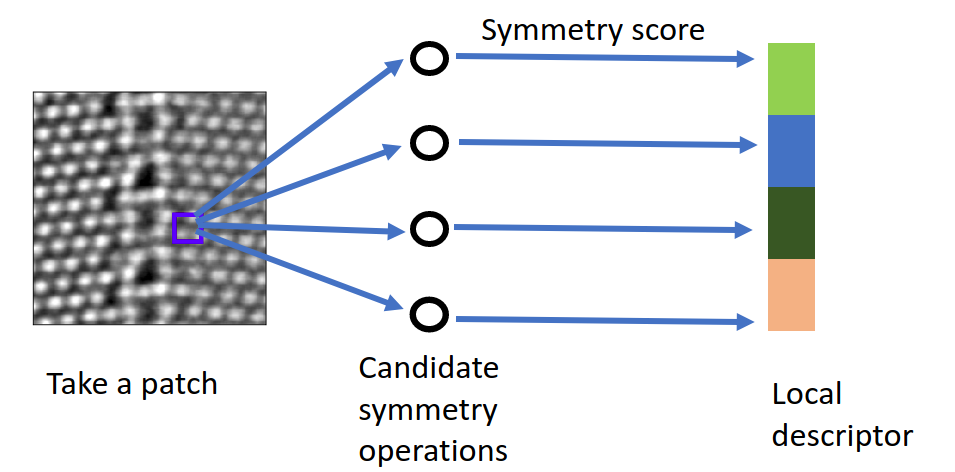
\includegraphics[width=1.\columnwidth]{schematic_diagram_local_descriptors.png}
\caption{A schematic diagram to illustrate the symmetry-based local descriptors. There are four local-symmetry-feature extractors corresponding to four candidate symmetry operations in this diagram. We obtain the local descriptors of length four containing four symmetry features.} 
\label{local_descriptors}
\end{figure}
%As we discussed above
We expect the symmetry score to measure the similarity between the original and the transformed patches. The Pearson's correlation coefficient is a good choice for this purpose, which takes a value in the range from -1 to 1 and and a larger value for the stronger similarity. For the original patch $P_{x,y}$ centered at the pixel $(x,y)$, and the corresponding transformed patch $OP_{x,y}$ by the operation $O$, the cross-correlation coefficient is evaluated according to 
\begin{widetext}
\begin{equation}\label{symmetry_score}
\begin{aligned}
\mathrm{SC}_O(x,y)  &\equiv \mathrm{Corr}\left( P_{x,y}, OP_{x,y} \right) \\
& =  \frac{\sum_{i=1}^{p_x}\sum_{j=1}^{p_y}[P_{x,y}(i,j)-\mu_{P_{x,y}}]\cdot OP_{x,y}(i,j)-\mu_{OP_{x,y}}{}]}{\sqrt{\sum_{i=1}^{p_x}\sum_{j=1}^{p_y}[P_{x,y}(i,j)-\mu_{P_{x,y}}]^2} \cdot \sqrt{\sum_{i=1}^{p_x}\sum_{j=1}^{p_y}[OP_{x,y}(i,j)-\mu_{OP_{x,y}}]^2} },
\end{aligned}
\end{equation}
\end{widetext}
where $O$ is an arbitrary symmetry operation, $P_{x,y}$ the original patch centered at $(x,y)$, $OP_{x,y}$ the transformed patch. Both patches have a size of $(p_x, p_y)$.  $P_{x,y}(i,j)$ and $P_{x,y}(i,j)$ are the intensities at the position $(i,j)$ in their relative coordinates. $\mu_{P_{x,y}}$ and $\mu_{OP_{x,y}}$  are the mean intensities of the patches $P_{x,y}$ and $OP_{x,y}$.  We emphasize that the relative coordinate is not necessarily the Cartesian coordinates, and it is more convenient to employ the polar coordinate to handle the rotation and reflection operations.
\begin{figure}[htbp]
\centering
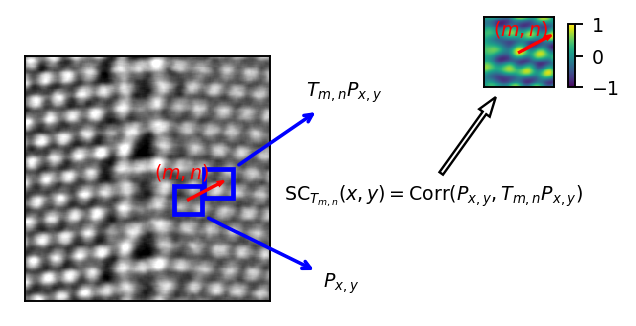
\includegraphics[width=1.\columnwidth]{schematic_diagram_local_correlation_map.png}
\caption{Computing the local descriptors at pixel $(x,y)$ based on the translation operations. The left plot: a real HAADF-STEM image of two copper grains. The right plot: the calculated local correlation map at pixel $(x,y)$. } 
\label{fig:local_correlation_map}
\end{figure}

In the remaining of this subsection, we employ the general procedure illustrated in Fig. \ref{local_descriptors} to obtain two group of local descriptors. The application to the translation operations gives us the local descriptors that have natural translational invariance within the same crystal pattern. In contrast, the local descriptors that are obtained by performing the rotation and reflection operations are not translationally invariant. We add a max-pooling step to enforce the translational invariance, similar to the treatment adopted in the convolutional neural networks \cite{Lecun2010}. 

\subsubsection{Extracting features via translation operations}
%After defining the similarity score, we next discuss how to select the candidate symmetry operations. Not all four types of symmetry operations are required to discriminate the crystal patterns in the microscopy image. 
If the crystal patterns have different lattice vectors or orientations, we only need the translation symmetries to discriminate them.
Based on the general procedure illustrated in Fig. \ref{local_descriptors}, we calculate the translational-symmetry-based local descriptors as follows. We denote the translation shift as $T_{m,n}$, which shifts the patch by $m$ pixels vertically and by $n$ pixels horizontally.  The transformed patch by this operation is simply the patch located at $(x+m, y+n)$, namely, $T_{m,n}P_{x,y} = P(x+m, y+n)$. 
Substituting this into Eq. \eqref{symmetry_score}, we obtain the symmetry score for the translation operation $T_{m,n}$,
\begin{equation}
    \mathrm{SC}_{T_{m,n}} (x,y) = \mathrm{Corr}(P_{x,y}, P_{x+m, y+n}).
\end{equation}
In practice, we confine the translation shift in a region of shape $(2w_x,2w_y)$, i.e.,  $|m|\leq w_x$ and  $ |n|\leq w_y$, and select uniformly a fixed number $N$ of translation shifts in this region. The symmetry scores for the selected translation shifts form a feature vector of length $N$, which is the local descriptor characterizing the local translational symmetries.  

Before we move on to the discussion of the rotation-reflection-based local descriptors, it is worthwhile to first analyze what crystal patterns the translational-symmetry-based local descriptors are suitable to discrimiate. Apparently, if the two crystal patterns have different Bravais lattices, lattice vectors, or orientations, we can employ the translational-symmety-based local descriptors to discriminate them easily. An interesting question is, can the translation-symmetry-based local descriptors discriminate easily the crystal patterns that have the same Bravais lattice, lattice vectors and orientation and different plane group symmetries? In order to answer this question, we take an extreme case in which we use all translation shifts in the region $ |m|\leq w_x$ and  $ |n|\leq w_y$ to form the local descriptors. In this case, the symmetry scores for all the translation shifts  forms a two-dimensional map of shape $(2w_x+1, 2w_y+1)$, as shown in Fig. \ref{fig:local_correlation_map}, which is denoted as the local correlation map in this paper. 
%The local correlation map is then reshaped into a one-dimensional vector, and become the local descriptors that characterize the translational symmetry in the vicinity of the pixel $(x,y)$. 
%The local descriptor has a high dimension if a large number of translation shifts are employed. The Principle component analysis is performed on the local descriptors of all pixels to reduce the dimension. 
%The local descriptors derived from the translation operations cannot represent all the symmetries of the crystal pattern, and therefore cannot discriminate all crystal patterns.  Clearly, if two crystal patterns have different Bravais lattices, different lattice vectors, or different crystal orientations, we can discriminate them with translation-operation-based local descriptors. The question is: if two crystal patterns have the same Bravais lattice, lattice vectors and orientation, can we still discriminate them with the translation-operation-based local descriptors? 
%In order to answer this question, we may analyze the symmetries of the local correlation map we introduced above, from which we obtain the local descriptors. 
As the entry in the local-correlation map is evaluated through the correlation coefficient between the original and the translationally-shifted patch, the local-correlation map has the same symmetry with the auto-correlation function of the crystal pattern. The symmetry of the auto-correlation function of the crystals is denoted as the Patterson symmetry in the X-ray diffraction community, \cite{ITA2002}, and we follow this convention in this paper. The relationship between the seventeen plane-group symmetries and the seven Patterson symmetries is presented in Table \ref{Patterson_symmetries} \cite{ITA2002}. The local-correlation map can only have seven Patterson symmetries because of the extra constraints. First, there is always a two-fold rotational axis at the center. Second, the glide-reflection symmetry is not allowed, and is replaced by the corresponding reflection symmetry. Clearly, if the two crystal patterns with the same lattice vectors and orientation have the same Patterson symmetry whereas different plane-group symmetries, it becomes difficult for the translational-symmetry-based local descriptors to discriminate them.  The other types of symmetries need to take into account for these microscopy images. 

%We thus draw a conclusion that the local descriptors based on the translation operations can discriminate the crystal patterns that have different Bravais lattices, lattice vectors, crystal orientations, or Patterson symmetries. If all of these are the same, we need to use the local descriptors based on other symmetry operations to discriminate crystal patterns. 
\begin{table*}[ht]
\centering
%\aptionsetup{width=1\textwidth}
\caption{The plane groups and the corresponding Patterson symmetries \cite{ITA2002}}
\label{Patterson_symmetries}
\begin{tabular}{ |p{6cm}|p{1cm}|p{1cm}|p{1cm}|p{1cm}|p{1cm}|p{1cm}|p{1cm}|p{1cm}|p{1cm}| }
\hline
 Plane group symmetry & p1 & p2 & p1m1 & p1g1 & p2mm & p2mg & p2gg & c1m1& c2mm  \\ 
\hline
 Corresponding Patterson symmetry & p2 & p2 & p2mm & p2mm  & p2mm & p2mm & p2mm & c2mm & c2mm \\
 \hline
 Plane group symmetry & p4& p4mm & p4gm & p3 & p6 & p3m1 & p31m  & p6mm &  \\
 \hline
 Corresponding Patterson symmetry & p4 & p4mm & p4mm & p6 & p6 & p6mm & p6mm  & p6mm &  \\
 \hline
 \end{tabular}
\end{table*}


\subsubsection{Extracting features via rotation and reflection operations}
%The rotation-reflection-based local descriptors can discriminate the crystal patterns that cannot be discriminated by the translation-based local descriptors. 
 %For example, the crystal patterns with space group p1m1, p1g1, p2mm, p2mg, and p2gg share the same Patterson symmetry p2mm and the same rectangular Bravais lattice. If the lattice vectors and the crystal orientation are also the same, it becomes impossible to discriminate them with the translation-based local descriptors. The rotation-based local descriptors can divide them into two groups, the one without two-fold rotation symmetry including p1m1 and p1g1, and the one with two-fold rotation symmetry including p2mm, p2mg, and p2gg. The reflection-based local descriptors can further discriminate them p1g1 and p2gg have no reflection symmetry, p2mg and p1m1 have parallel reflection planes, while p2mm has orthogonal reflection planes. 
Following the procedure shown in Fig. \ref{local_descriptors}, we present the implementation of the rotation-reflection-based local descriptors.  In this case, it is more convenient to take the circular patches and employ the polar coordinates. The patches are rotated by a specific angle or reflected by a specific plane, and the symmetry score is again the Pearson's correlation coefficient between the original and the transformed patches, according to Eq. \eqref{symmetry_score}. We select a series of rotation angles $\{\ang{60}, \ang{90}, \ang{120},\ang{180}\}$, and also a series of reflection planes, and the symmetry score for each candidate symmetry operation represents a specific rotation or reflection symmetry feature.
The local descriptors we obtain here cannot be used straightforwardly in the segmentation since they are not translationally invariant within the same crystal pattern.  We present an example for a given reflection symmetry operation in Fig. \ref{reflection_local_descriptors}. The symmetry scores show clearly different preferences to the crystal patterns on the left and right-hand sides.  However, the symmetry scores are not homogeneously distributed within the crystal pattern indicating the point-group nature of the reflection and rotation symmetries. 
We add the max-pooling step to enforce the translational invariance, similar to the treatment in the convolutional neural networks \cite{Lecun2010}. As the max-pooling does not contain training parameters, our segmentation approach is still kept free of training.
%and the principal component analysis is then used to reduced the dimensions and get the local descriptors that distribute smoothly, as shown in the last subplot in Fig. \ref{reflection_local_descriptors}. 

\begin{figure}[htbp]
\centering
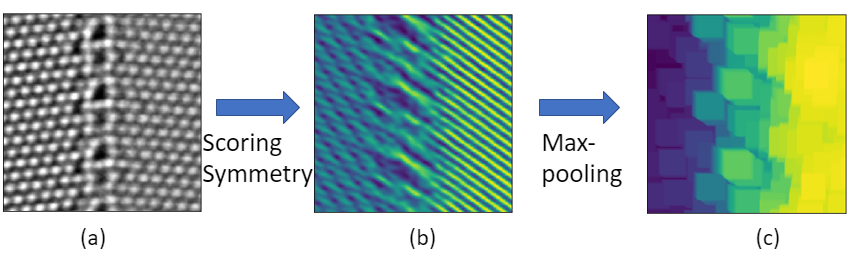
\includegraphics[width=1.\columnwidth]{reflection_descriptors.png}
\caption{An example to illustrate the calculation of reflection-based local descriptors. The rotation-based local descriptors can be obtained in the similar way. (a)  A real HAADF-STEM image of two copper grains. (b) The symmetry scores for a specific symmetry operation at all pixels. The color coding represents values of reflection symmetry scores. (c) The max-pooling enforces the translational invariance.}
%(d) PCA compresses all channels into smooth features. The data projected on the first principal component are plotted here. } 
\label{reflection_local_descriptors}
\end{figure}


\subsection{Principal component analysis}
The local descriptor is a high-dimensional feature vector with each channel characterizing a specific symmetry. We may combine the information of all channels to get several features that capture the main differences of the crystal patterns in the image, and use these features as the input of the K-means clustering. With this treatment, we drop out the noisy information that is not important to discriminate the crystal patterns and reduce the computational cost in the latter clustering. 
In practice, we maximize an empirical metric, the variance, to obtain the optimal features. Intuitively, the larger the variance of the feature is, the more separate the crystal patterns are in the corresponding feature space. This metric works to obtain the optimal features in our case simply because the correlation between the separability and the variance of the features in our local descriptors, and a detailed discussion will be seen in section \ref{discussion}.
%This metric works for the segmentation in our case,
If we further assume that the optimal feature is a linear combination of all channels in the local descriptor, with the Euclidean norm of the combination coefficients bounded to be one, we immediately see that we can obtain them by simply projecting the local descriptors onto the principal components in PCA. We denote the optimal features obtained in this way as the PCA features, and employ the implementation of PCA in scikit-learn \cite{scikit-learn} in our code.

\subsection{K-means clustering}
We feed the PCA features into the k-means clustering algorithm \cite{kmeans1967, kmeans2007} to cluster the pixels in the feature space, which finds the cluster centers by minimizing the within-cluster variance and partition the feature space into Voronoi cells.  Each cluster corresponds to a specific crystal pattern, and the pixels grouped into the same cluster are assigned with the same pattern label.  We employ the implementation of the k-means clustering in scikit-learn \cite{scikit-learn} in our code, and the cluster centers are first initialized randomly and then optimized in an iterative way. The number of clusters is the hyperparameter that needs to be specified by the users. 

\subsection{Stride and upsampling}
In many cases, it is not necessary to calculate the local descriptors of all pixels as they are highly correlated. We may first use the stride scheme to downsample the image, and then perform upsampling after the clustering is finished in order to match the size of the original image. In this way, we can reduce the computational cost drastically.  The stride scheme we employed is the same with the one used in the convolutional neural networks. To be more specific,  in the first step of our approach,
instead of calculating the local descriptors for each pixel by shifting the local-symmetry-feature extractors every time by one unit, we shift them by a step size of $s_x$ units vertically and by a step size of $s_y$ units horizontally and only calculate the local descriptors for a fraction of the pixels. As the image is downsampled by the stride scheme, we add an upsampling scheme after the k-means clustering to expand the segmented image. We in the end obtain the segmented image that have the same size with the original one. In our upsampling scheme, we simply do an interpolation for the pixels that are not clustered based on the pattern labels of the clustered pixels, and the interpolated values are then rounded to integers.We note that both the stride scheme and the upsampling scheme contain no training parameters, which keeps our whole approach free of training.  
%Apparently, the step size influences the spatial resolution and the computational cost significantly. A large (small) step size leads to the cheap (expensive) computational cost and low (high) resolution.   
\section{Application and discussion}\label{discussion}
In Fig. \ref{fig:FeNb_phase_boundary}, we present an application to the HAADF-STEM image containing two phases ($\mu$ phase and Laves phase) of the iron-niobium intermetallics. Their crystal patterns in the specific projection plane have different two-dimensional Bravais lattices, one with the oblique lattice and the other with the rectangular lattice. The translation-symmetry-based local descriptors are adequate to discriminate them. We select uniformly one hundred translation operations in the region $|m|<150$ pixels and $|n|<150$ pixels to generate the local descriptors. The pattern labels are correctly assigned to the pixels in the upper and lower half of the image, as shown in Fig. \ref{fig:FeNb_phase_boundary}. 
\begin{figure}
    \centering
    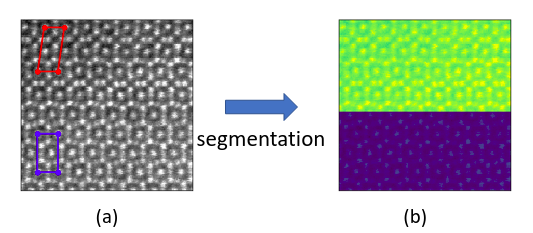
\includegraphics[width=1.\columnwidth]{FeNb_raw_and_segmented_images.png}
    \caption{(a) A HAADF-STEM image of two phases ($\mu$ phase and Laves phase) of the iron-niobium intermetallics that have different Bravais lattices. The unit cells of the two phases are shown in red and blue.  (b) The image superimposed of the HAADF intensity and the pattern labels.  }
    \label{fig:FeNb_phase_boundary}
\end{figure}

\begin{figure}
    \centering
    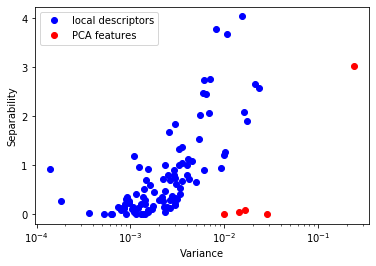
\includegraphics[width=0.8\columnwidth]{separability_and_variance.png}
    \caption{ The separability and variance of all features in the local descriptors and the five PCA features.  }
    \label{fig:separability_and_variance}
\end{figure}
We use this example to illustrate why our segmentation approach can work in an unsupervised manner. In order to show this, we calculate the Fisher separability \cite{Fisher1936} and variance for all features in the local descriptors and the five PCA features with largest variances. The Fisher separability is defined as the ratio between the between-class variance and the within-class variance \cite{Fisher1936}, and can be evaluated according to
\begin{equation}
    S = \frac{N_1(\mu_1-\mu)^2 + N_2(\mu_2-\mu)^2}{
    N_1\sigma_1^2 + N_2 \sigma_2^2},
\end{equation}
where $N_1$ and $N_2$ are the number of samples in the first and the second class, $\mu_1$ and $\mu_2$ the within-class means, $\mu$ the total mean, and $\sigma_1$ and $\sigma_2$ the within-class variances. The separability tells how well the feature can discriminate the two crystal patterns, and the variance dictates the energy of the feature. We see that there is a strong correlation between the separability and the variance. The feature that has a larger variance also has a better separability. 
%The PCA features also have the similar trend. 
The PCA doesn't increase the separability, whereas it makes the energy more concentrated on the features that have better separability. We might think of the features with good separability the signal and those with bad separability the noise. The correlation between the separability and the variance is crucial for the unsupervised approach, which results in a good signal-noise ratio and the successful segmentation.   
\begin{figure}
    \centering
    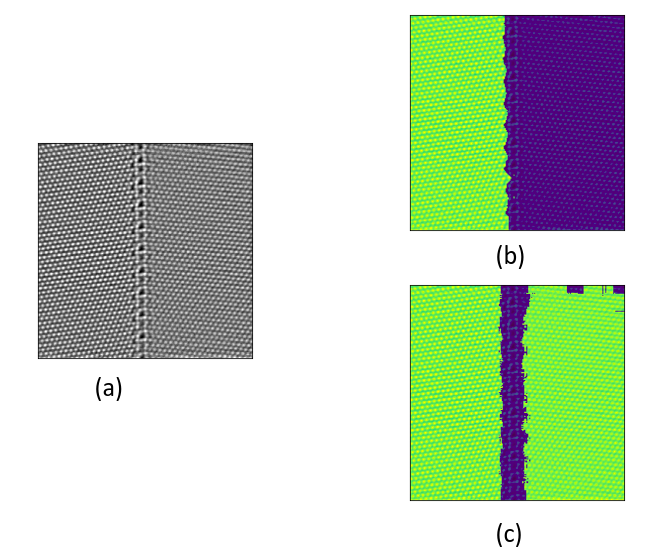
\includegraphics[width=0.8\columnwidth]{Cu_grain_boundary.png}
    \caption{ (a) HAADF-STEM image containing two Cu single-crystal grains and a tilt grain boundary. (b) Segmentation via the reflection-based local descriptors. The image is superimposed of the HAADF intensity and the class labels. (c) Segmentation via the rotation-based local descriptors. The image is superimoposed of the HAADF intensity and the pattern labels.   }
    \label{fig:Cu_grain_boundary}
\end{figure}

We show the second example in Fig. \ref{fig:Cu_grain_boundary}, in which we segment the HAADF-STEM image containing two differently oriented copper crystal grains and one tilt grain boundary with the reflection-symmetry-based and the rotation-symmetry-based local descriptors separately. The reflection-symmetry-based local descriptors partition this image into two segments, and the left and right crystal grains are clearly separated from each other. In contrast,  the rotation-symmetry-based local descriptors group the two crystal grains into the same crystal pattern, and the crystal boundary is segmented into a different crystal pattern. 
The results indicate the influence of the choice of the local descriptors, as different local descriptors capture different symmetry information. In this example, the reflection-symmetry-based local descriptors are not rotationally invariant, and therefore, the same crystal grains with different orientations are partitioned into different crystal patterns. In contrast, the rotation-symmetry-based local descriptors are rotationally invariant and result in different interpretation of the crystal patterns in the image.

\begin{figure}
    \centering
    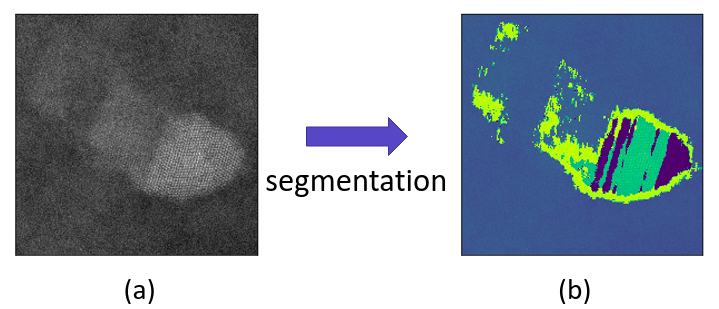
\includegraphics[width=0.8\columnwidth]{nickel_precipitate.png}
    \caption{ (a) HAADF-STEM image for a nickel precipitate containing twin bounaries and stacking faults. (b) Image superimposed of the HAADF intensity and the pattern labels.   }
    \label{fig:nickel_precipitate}
\end{figure}

In our third example shown in Fig. \ref{fig:nickel_precipitate}, we segment the HAADF-STEM image for a nickel precipitate containing twin boundaries and stacking faults. We observed a very good spacial resolution, and the stacking faults and the twin boundaries are much better visible in the segmented image than in the original one.

We provide the jupyter notebooks for the calculations in this section \cite{pystem}, and all the figures might be reproduced with little effort. 

%The microscopy images in all the three examples have a size of 1024x1024 pixels, and the segmentation took several seconds on a laptop computer (Intel(R) Core(TM) i5-7200U CPU @ 2.50GHz). Each figures in this section can be reproduced by the jupyter notebooks in our github repository . 

%The users need to choose the proper local descriptors based on4 teir purpose, which seems the drawback of the unsupervised approach. At the same time, it gives the users the freedom to get the desired interpretation. 
%as the two crystal grains have the same rotation symmetry and the crystal boundary has a different one. As the segmentation results depend on the choice of the local descriptorsAt the same time, it gives the users the freedom to get the desired segmentation results based on their purpose, which is an advantage of this approach. 
%we show that the segmentation results have strong dependence on the choice of local descriptors. In the HAADF-STEM image of this example, there are two crystal grains with different orientations and a tilt grain boundary in between. 


\section{Conclusion}
We present a semi-automated unsupervised machine-learning approach to segment the atomic-resolution microscopy images. In our approach, we extract the local descriptor via the symmetry operations, which forms an abundance feature vector to characterize the local symmetry information. We then use the principal component analysis (PCA) to reduce the dimension of the local descriptors, and observe in our example that the energy of the features with good separability is indeed increased by PCA. After that, we feed the PCA features into the k-means clustering algorithm in order to assign the pattern labels to the pixels. A stride and upsampling scheme is proposed in order to reduce the computational cost.
We presented the successful application to the experimental HAADF-STEM images, and revealed one important feature of the unsupervised segmentation approach, the strong correlation between the feature's separability and energy (variance).  
We packaged our code as a python module, and released it in the github \cite{github} and the python repository \cite{pystem}. More tests can be found in the example folder in our github repository. 


%We cannot employ the pixel intensity directly as the symmetry are not represented by the intensity of one single pixel. The local descriptors (features) that characterize the symmetries of the structures are thus required. There are four types of symmetry in the two-dimensional structures, the translation, rotation, reflection and glide-reflection.
%which lead to the seventeen plane groups. Ideally, the local descriptors should be able to discriminate any pairs of them. 
%Correspondingly, we introduce four types of local descriptors in the subsection \ref{local_descriptors}. We then give a brief introduction to the dimension reduction and the clustering algorithms. After that, we present our unsampling scheme in order to match the shapes of the segmented and the original images and finalize our segmentation approach. 

%\subsection{Symmetry-based local %descriptors}\label{local_descriptors}
%In this subsection, we target at developing local descriptors that characterize the symmetries of the local surrounding of a given pixel $(x,y)$.    
%We first present the translational-symmetry-based local descriptors. After that we show the other three types of descriptors.  
%Our procedure to develop the symmetry-based local descriptors is: we first quantify the symmetry for a specific  ,   

%To quantify the local symmetry 
%in the vicinity of the given pixel $(x,y)$ 
%for a specific symmetry operation $O$, 
%in a microscopy image of shape $(X,Y)$,
%we introduce a symmetry indicator $\mathrm{SI}_O(x,y)$ that is defined as the similarity between the patch centered at $(x,y)$, and the corresponding transformed patch by the symmetry operation $O$.
%The original and transformed patches are denoted as $P_{x,y}$ and $OP_{x,y}$, respectively. The symmetry operation $O$ might be the translation $T$, rotation $R$, reflection $M$, or the glide reflection $G$. 
%There are various choices to quantify the similarity, and in our case, we adopt the correlation coefficient,

%The local-correlation-map descriptors characterizes the local translational symmetry. They are well suited to segment the image in which the structures have different translational symmetries. However, if the structures have the same translational symmetry and are different in terms of other symmetries, the local-correlation-map descriptors are not sufficient to differentiate them. In these cases, the local descriptors based on other symmetries are required. We next present the local descriptors that characterize the rotational, reflectional, and glide-reflection symmetries. 
%Their are various ways to define the similarity distance, and in our case, we employ the correlation coefficient, 



%Many of the previous attempts for segmenting microscopy images were made in the community of biology \cite{Navlakha2013, Ignacio2017,Belevich2016,Dang2019}, which are not straightforwardly applicable for materials-science images,  while a few made in the materials-science community  

\bibliography{literature}
\bibliographystyle{apsrev}





%We first represent the symmetry by the self-similarity-based symmetry indicators, and then combine the indicators to define the local descriptors. 
%We assume that the image has a shape of $(X,Y)$, and we define the intensity of the pixel $(x,y)$ as $I(x,y)$, where $x$ goes from the 1 to $X$, and $y$ goes from 1 to $Y$.  
%For the translational symmetry w.r.t. the shift $(m,n)$, we have the invariance below in the ideal case, 
%\begin{equation}
%    I(x+m, y+n) = I(x, y).
%\end{equation}
%We take two patches of shape $(p_x,p_y)$ centered at $(x,y)$ and $(x+m, y+n)$ and denote them as $P(x,y)$ and $P(x+m, y+n)$. Due to the translational invariance w.r.t. the shift $(m,n)$, they have strong similarity (identical in the ideal case). We employ the correlation coefficient to represent the similarity and define the translational similarity indicator (TSI),
%\lipsum[1]
%\begin{widetext}
%\begin{equation}
%\begin{aligned}
%\mathrm{TSI}^{(m,n)}_{(x,y)}  &\equiv \mathrm{Corr}\left[ P(x,y), P(x+m,y+n) \right] \\
%& =  \frac{\sum_{i=1}^{p_x}\sum_{j=1}^{p_y}[I(x+i,y+j)-\mu_p(x,y)]\cdot [I(x+m+i,y+n+j)-\mu_p(x+m,y+n)]}{\sqrt{\sum_{i=1}^{p_x}\sum_{j=1}^{p_y}[I(x+i,y+j)-\mu_p(x,y)]^2} \cdot \sqrt{\sum_{i=1}^{p_x}\sum_{j=1}^{p_y}[I(x+m+i,y+n+j)-\mu_p(x+m,y+n)]^2}},
%\end{aligned}
%\end{equation}
%\end{widetext}
%where $\mu_p(x,y)$ and $\mu_p(x+m,y+n)$ are the mean intensities of the patches $P(x,y)$ and $P(x+m, y+n)$, respectively. The TSI takes a value in the range from $-1$ to $1$. The larger it is, the stronger symmetry it indicates.  
\end{document}